\documentclass[11pt]{article}
\usepackage{cornell-notes}
\usepackage{mathtools}
\usepackage{needspace}
\usepackage{ragged2e}
\usepackage{adjustbox}
\usepackage{tikz}
\usetikzlibrary{arrows.meta,positioning}
\tcbuselibrary{most}
\geometry{letterpaper,margin=0.72in,headheight=15pt}
\setCornellCollection{Calculus Cornell Notes}
\setCornellUnitType{Chapter}
\setCornellUnitNumber{3}
\setCornellUnitTitle{Applications of Differentiation}

\definecolor{Ink}{HTML}{17324D}
\definecolor{Teal}{HTML}{147D78}
\definecolor{Sky}{HTML}{DDEEF1}
\definecolor{Cue}{HTML}{EEF2F5}
\definecolor{Warm}{HTML}{FFF3D6}
\definecolor{Alert}{HTML}{9D3C32}
\definecolor{Green}{HTML}{276749}
\definecolor{Rule}{HTML}{AAB8C2}
\hypersetup{colorlinks=true,linkcolor=Ink,urlcolor=Teal,pdfborder={0 0 0}}
\setlength{\parindent}{0pt}
\setlength{\parskip}{4pt}
\setlist{nosep,leftmargin=*}
\titleformat{\section}{\Large\bfseries\color{Ink}}{}{0pt}{}[\color{Teal}\titlerule]
\titleformat{\subsection}{\large\bfseries\color{Teal}}{}{0pt}{}
\pagestyle{fancy}
\fancyhf{}
\fancyhead[L]{\small\color{Ink}\textsc{Cornell Notes}}
\fancyhead[R]{\small\color{Teal}\nouppercase{\leftmark}}
\fancyfoot[L]{\footnotesize\color{Ink}Active recall $\bullet$ Worked reasoning $\bullet$ Verification}
\fancyfoot[R]{\footnotesize\color{Ink}\thepage\ of \pageref*{LastPage}}
\renewcommand{\headrulewidth}{0.5pt}
\renewcommand{\footrulewidth}{0.4pt}
\newcolumntype{Y}{>{\RaggedRight\arraybackslash}X}
\newtcolorbox{orientationbox}{enhanced,breakable,colback=Sky,colframe=Teal,boxrule=0.7pt,arc=2mm,title=Chapter orientation,fonttitle=\bfseries}
\newtcolorbox{sectionsummarybox}{enhanced,breakable,colback=white,colframe=Teal,boxrule=0.6pt,arc=1.5mm,left=2mm,right=2mm,top=1mm,bottom=1mm,title=Section synthesis,fonttitle=\bfseries\color{Teal}}
\newtcolorbox{warningbox}{enhanced,breakable,colback=Warm,colframe=Alert,boxrule=0.7pt,arc=1.5mm,title=Common error audit,fonttitle=\bfseries}
\newtcolorbox{checkbox}{enhanced,breakable,colback=white,colframe=Green,boxrule=0.7pt,arc=1.5mm,title=Verification habit,fonttitle=\bfseries}
\newcommand{\cornellcuehead}{\rowcolor{Ink}\color{white}\bfseries Cue / recall prompt & \color{white}\bfseries Notes / reasoning \\\endhead}
\newcommand{\cornellcuerow}[2]{\rowcolor{Cue}#1 & #2 \\\addlinespace[3pt]}
% Table-safe: delegates to the shared Cornell formula box (cornell-notes.sty),
% which cannot emit \pagebreak/\noalign inside longtable cells.
\newcommand{\formula}[1]{\CornellFormula[colback=Sky,colframe=Teal]{#1}}

\title{Chapter 3: Applications of Differentiation\\[2mm]\large Cornell Notes}
\author{}
\date{}
\hypersetup{pdftitle={Chapter 3: Applications of Differentiation - Cornell Notes},pdfauthor={},pdfsubject={Calculus study notes},pdfkeywords={calculus, Cornell notes, active recall}}
\begin{document}
\maketitle
\thispagestyle{fancy}
\begin{orientationbox}
Use derivatives to prove qualitative behavior, sketch functions, solve optimization problems, approximate roots, and quantify local error. These notes follow the complete local section sequence (165--246) and emphasize definitions, governing results, strategy selection, and verifiable reasoning.
\end{orientationbox}

\section{Prerequisite map}
\begin{minipage}[t]{0.42\textwidth}
\textbf{Bring forward}
\begin{itemize}
\item Derivative rules
\item Continuity
\item Function domains
\item Algebraic equation solving
\end{itemize}
\end{minipage}\hfill
\begin{minipage}[t]{0.54\textwidth}
\textbf{Chapter flow}
\begin{center}
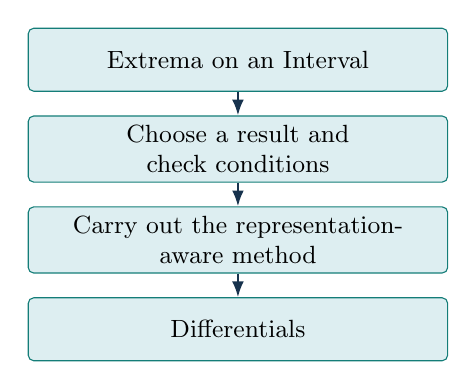
\begin{tikzpicture}[node distance=3mm, every node/.style={font=\small,align=center}, box/.style={draw=Teal,rounded corners=2pt,fill=Sky,minimum height=8mm,text width=0.42\textwidth}, arr/.style={-{Latex[length=2mm]},thick,draw=Ink}]
\node[box] (a) {Extrema on an Interval};
\node[box,below=of a] (b) {Choose a result and check conditions};
\node[box,below=of b] (c) {Carry out the representation-aware method};
\node[box,below=of c] (d) {Differentials};
\draw[arr] (a)--(b); \draw[arr] (b)--(c); \draw[arr] (c)--(d);
\end{tikzpicture}
\end{center}
\end{minipage}

\section{Learning objectives}
\begin{enumerate}
\item Explain the central objects and hypotheses in 3.1 and 3.9.
\item Translate among algebraic, graphical, numerical, and verbal representations.
\item Select an appropriate formula or theorem before beginning symbolic work.
\item Carry out multi-step calculations while preserving domain, sign, orientation, and units.
\item Diagnose common errors by testing assumptions and checking the result independently.
\item Synthesize the chapter's methods into a reusable problem-solving workflow.
\end{enumerate}

\section{3.1 Extrema on an Interval}
\begin{longtable}{C N}\cornellcuehead
\cornellcuerow{What is the governing idea in 3.1?}{Absolute extrema on a closed interval occur among critical numbers and endpoints when the function is continuous.}
\cornellcuerow{Which result should be recalled?}{\formula{f'(c)=0\ \text{or}\ f'(c)\ \text{does not exist}}}
\cornellcuerow{How should a problem be organized?}{Find critical numbers in the domain, evaluate the function at them and at endpoints, then compare actual function values.}
\cornellcuerow{What should be checked before accepting an answer?}{Confirm the hypotheses and domain, preserve units and orientation when relevant, and substitute or differentiate back into the defining relation.}
\end{longtable}
\begin{warningbox}A critical number is only a candidate; ignoring endpoints or points where $f'$ is undefined can miss the absolute extremum.\end{warningbox}
\begin{sectionsummarybox}Absolute extrema on a closed interval occur among critical numbers and endpoints when the function is continuous. The operational habit is to find critical numbers in the domain, evaluate the function at them and at endpoints, then compare actual function values.\end{sectionsummarybox}
\section{3.2 Rolle's Theorem and the Mean Value Theorem}
\begin{longtable}{C N}\cornellcuehead
\cornellcuerow{What is the governing idea in 3.2?}{Under continuity and differentiability hypotheses, a secant slope is attained by at least one tangent slope.}
\cornellcuerow{Which result should be recalled?}{\formula{f'(c)=\frac{f(b)-f(a)}{b-a}}}
\cornellcuerow{How should a problem be organized?}{Verify continuity on $[a,b]$ and differentiability on $(a,b)$ before solving the theorem's derivative equation.}
\cornellcuerow{What should be checked before accepting an answer?}{Confirm the hypotheses and domain, preserve units and orientation when relevant, and substitute or differentiate back into the defining relation.}
\end{longtable}
\begin{warningbox}The conclusion is not licensed when a corner, discontinuity, or domain gap violates a hypothesis.\end{warningbox}
\begin{sectionsummarybox}Under continuity and differentiability hypotheses, a secant slope is attained by at least one tangent slope. The operational habit is to verify continuity on $[a,b]$ and differentiability on $(a,b)$ before solving the theorem's derivative equation.\end{sectionsummarybox}
\section{3.3 Increasing and Decreasing Functions and the First Derivative Test}
\begin{longtable}{C N}\cornellcuehead
\cornellcuerow{What is the governing idea in 3.3?}{The sign of $f'$ partitions the domain into intervals of increase and decrease and classifies sign-changing critical points.}
\cornellcuerow{Which result should be recalled?}{\formula{f'>0\Rightarrow f\text{ increases},\qquad f'<0\Rightarrow f\text{ decreases}}}
\cornellcuerow{How should a problem be organized?}{Create a sign chart using domain breaks and critical numbers, test one point per interval, and read local extrema from sign changes.}
\cornellcuerow{What should be checked before accepting an answer?}{Confirm the hypotheses and domain, preserve units and orientation when relevant, and substitute or differentiate back into the defining relation.}
\end{longtable}
\begin{warningbox}Testing only $f'(c)=0$ cannot distinguish a turning point from a stationary point with no extremum.\end{warningbox}
\begin{sectionsummarybox}The sign of $f'$ partitions the domain into intervals of increase and decrease and classifies sign-changing critical points. The operational habit is to create a sign chart using domain breaks and critical numbers, test one point per interval, and read local extrema from sign changes.\end{sectionsummarybox}
\section{3.4 Concavity and the Second Derivative Test}
\begin{longtable}{C N}\cornellcuehead
\cornellcuerow{What is the governing idea in 3.4?}{The sign of $f''$ describes how slopes change; an inflection point requires a change in concavity.}
\cornellcuerow{Which result should be recalled?}{\formula{f''>0\Rightarrow\text{concave up},\qquad f''<0\Rightarrow\text{concave down}}}
\cornellcuerow{How should a problem be organized?}{Find candidates from $f''=0$ or undefined, build a second-derivative sign chart, and confirm that the function is defined at any claimed inflection point.}
\cornellcuerow{What should be checked before accepting an answer?}{Confirm the hypotheses and domain, preserve units and orientation when relevant, and substitute or differentiate back into the defining relation.}
\end{longtable}
\begin{warningbox}$f''(c)=0$ alone neither proves an inflection point nor classifies every critical point.\end{warningbox}
\begin{sectionsummarybox}The sign of $f''$ describes how slopes change; an inflection point requires a change in concavity. The operational habit is to find candidates from $f''=0$ or undefined, build a second-derivative sign chart, and confirm that the function is defined at any claimed inflection point.\end{sectionsummarybox}
\section{3.5 Limits at Infinity}
\begin{longtable}{C N}\cornellcuehead
\cornellcuerow{What is the governing idea in 3.5?}{End behavior is governed by dominant growth; finite limits at infinity determine horizontal asymptotes.}
\cornellcuerow{Which result should be recalled?}{\formula{\lim_{x\to\pm\infty}\frac{a_mx^m+\cdots}{b_nx^n+\cdots}}}
\cornellcuerow{How should a problem be organized?}{Divide rational functions by the highest denominator power and compare degrees and leading coefficients.}
\cornellcuerow{What should be checked before accepting an answer?}{Confirm the hypotheses and domain, preserve units and orientation when relevant, and substitute or differentiate back into the defining relation.}
\end{longtable}
\begin{warningbox}A horizontal asymptote describes end behavior and may be crossed; it is not a forbidden line.\end{warningbox}
\begin{sectionsummarybox}End behavior is governed by dominant growth; finite limits at infinity determine horizontal asymptotes. The operational habit is to divide rational functions by the highest denominator power and compare degrees and leading coefficients.\end{sectionsummarybox}
\section{3.6 A Summary of Curve Sketching}
\begin{longtable}{C N}\cornellcuehead
\cornellcuerow{What is the governing idea in 3.6?}{A reliable sketch integrates domain, intercepts, symmetry, asymptotes, monotonicity, extrema, concavity, and inflection behavior.}
\cornellcuerow{Which result should be recalled?}{\formula{f,\ f',\ f''\quad\text{provide complementary evidence}}}
\cornellcuerow{How should a problem be organized?}{Build one ordered feature table, place verified anchors, and connect them in a way consistent with all sign charts and limits.}
\cornellcuerow{What should be checked before accepting an answer?}{Confirm the hypotheses and domain, preserve units and orientation when relevant, and substitute or differentiate back into the defining relation.}
\end{longtable}
\begin{warningbox}Plotting isolated points without reconciling derivative signs often creates a visually plausible but logically impossible curve.\end{warningbox}
\begin{sectionsummarybox}A reliable sketch integrates domain, intercepts, symmetry, asymptotes, monotonicity, extrema, concavity, and inflection behavior. The operational habit is to build one ordered feature table, place verified anchors, and connect them in a way consistent with all sign charts and limits.\end{sectionsummarybox}
\section{3.7 Optimization Problems}
\begin{longtable}{C N}\cornellcuehead
\cornellcuerow{What is the governing idea in 3.7?}{Optimization converts a contextual objective and constraints into a one-variable extremum problem.}
\cornellcuerow{Which result should be recalled?}{\formula{\text{optimize }Q(x)\text{ subject to the feasible domain}}}
\cornellcuerow{How should a problem be organized?}{Define variables with units, write the objective, eliminate extra variables with constraints, determine the feasible interval, and compare candidates.}
\cornellcuerow{What should be checked before accepting an answer?}{Confirm the hypotheses and domain, preserve units and orientation when relevant, and substitute or differentiate back into the defining relation.}
\end{longtable}
\begin{warningbox}Solving $Q'=0$ without checking feasibility, endpoints, or the requested quantity can select a nonphysical answer.\end{warningbox}
\begin{sectionsummarybox}Optimization converts a contextual objective and constraints into a one-variable extremum problem. The operational habit is to define variables with units, write the objective, eliminate extra variables with constraints, determine the feasible interval, and compare candidates.\end{sectionsummarybox}
\section{3.8 Newton's Method}
\begin{longtable}{C N}\cornellcuehead
\cornellcuerow{What is the governing idea in 3.8?}{Newton iteration replaces a curve locally by its tangent to approximate a zero.}
\cornellcuerow{Which result should be recalled?}{\formula{x_{n+1}=x_n-\frac{f(x_n)}{f'(x_n)}}}
\cornellcuerow{How should a problem be organized?}{Choose a sensible initial estimate, iterate while $f'$ remains safe, and verify convergence by residual and successive-change checks.}
\cornellcuerow{What should be checked before accepting an answer?}{Confirm the hypotheses and domain, preserve units and orientation when relevant, and substitute or differentiate back into the defining relation.}
\end{longtable}
\begin{warningbox}A small derivative or poor starting point can cause divergence, cycling, or convergence to an unintended root.\end{warningbox}
\begin{sectionsummarybox}Newton iteration replaces a curve locally by its tangent to approximate a zero. The operational habit is to choose a sensible initial estimate, iterate while $f'$ remains safe, and verify convergence by residual and successive-change checks.\end{sectionsummarybox}
\section{3.9 Differentials}
\begin{longtable}{C N}\cornellcuehead
\cornellcuerow{What is the governing idea in 3.9?}{The differential gives a local linear estimate of output change and supports propagated-error approximations.}
\cornellcuerow{Which result should be recalled?}{\formula{dy=f'(x)\,dx,\qquad \Delta y\approx dy}}
\cornellcuerow{How should a problem be organized?}{Identify the base point and small input change, compute the derivative there, and distinguish the exact change from its linear estimate.}
\cornellcuerow{What should be checked before accepting an answer?}{Confirm the hypotheses and domain, preserve units and orientation when relevant, and substitute or differentiate back into the defining relation.}
\end{longtable}
\begin{warningbox}The approximation is local; a large $dx$ or rapidly changing derivative can make $dy$ unreliable.\end{warningbox}
\begin{sectionsummarybox}The differential gives a local linear estimate of output change and supports propagated-error approximations. The operational habit is to identify the base point and small input change, compute the derivative there, and distinguish the exact change from its linear estimate.\end{sectionsummarybox}

\section{Definitions and theorem register}
\small
\begin{longtable}{@{}>{\RaggedRight\arraybackslash}p{0.24\textwidth}>{\RaggedRight\arraybackslash}p{0.40\textwidth}>{\RaggedRight\arraybackslash}p{0.29\textwidth}@{}}
\toprule
\textbf{Topic} & \textbf{Meaning and conditions} & \textbf{Canonical form}\\
\midrule\endhead
3.1 Extrema on an Interval & Absolute extrema on a closed interval occur among critical numbers and endpoints when the function is continuous. & \adjustbox{max width=\linewidth}{\(\displaystyle f'(c)=0\ \text{or}\ f'(c)\ \text{does not exist}\)} \\\addlinespace[2pt]
3.2 Rolle's Theorem and the Mean Value Theorem & Under continuity and differentiability hypotheses, a secant slope is attained by at least one tangent slope. & \adjustbox{max width=\linewidth}{\(\displaystyle f'(c)=\frac{f(b)-f(a)}{b-a}\)} \\\addlinespace[2pt]
3.3 Increasing and Decreasing Functions and the First Derivative Test & The sign of $f'$ partitions the domain into intervals of increase and decrease and classifies sign-changing critical points. & \adjustbox{max width=\linewidth}{\(\displaystyle f'>0\Rightarrow f\text{ increases},\qquad f'<0\Rightarrow f\text{ decreases}\)} \\\addlinespace[2pt]
3.4 Concavity and the Second Derivative Test & The sign of $f''$ describes how slopes change; an inflection point requires a change in concavity. & \adjustbox{max width=\linewidth}{\(\displaystyle f''>0\Rightarrow\text{concave up},\qquad f''<0\Rightarrow\text{concave down}\)} \\\addlinespace[2pt]
3.5 Limits at Infinity & End behavior is governed by dominant growth; finite limits at infinity determine horizontal asymptotes. & \adjustbox{max width=\linewidth}{\(\displaystyle \lim_{x\to\pm\infty}\frac{a_mx^m+\cdots}{b_nx^n+\cdots}\)} \\\addlinespace[2pt]
3.6 A Summary of Curve Sketching & A reliable sketch integrates domain, intercepts, symmetry, asymptotes, monotonicity, extrema, concavity, and inflection behavior. & \adjustbox{max width=\linewidth}{\(\displaystyle f,\ f',\ f''\quad\text{provide complementary evidence}\)} \\\addlinespace[2pt]
3.7 Optimization Problems & Optimization converts a contextual objective and constraints into a one-variable extremum problem. & \adjustbox{max width=\linewidth}{\(\displaystyle \text{optimize }Q(x)\text{ subject to the feasible domain}\)} \\\addlinespace[2pt]
3.8 Newton's Method & Newton iteration replaces a curve locally by its tangent to approximate a zero. & \adjustbox{max width=\linewidth}{\(\displaystyle x_{n+1}=x_n-\frac{f(x_n)}{f'(x_n)}\)} \\\addlinespace[2pt]
3.9 Differentials & The differential gives a local linear estimate of output change and supports propagated-error approximations. & \adjustbox{max width=\linewidth}{\(\displaystyle dy=f'(x)\,dx,\qquad \Delta y\approx dy\)} \\\addlinespace[2pt]
\bottomrule
\end{longtable}
\normalsize

\section{Formula and method sheet}
\small
\begin{longtable}{@{}>{\RaggedRight\arraybackslash}p{0.08\textwidth}>{\RaggedRight\arraybackslash}p{0.48\textwidth}>{\RaggedRight\arraybackslash}p{0.37\textwidth}@{}}
\toprule
\textbf{Sec.} & \textbf{Method sequence} & \textbf{Stop-and-check trigger}\\
\midrule\endhead
3.1 & Find critical numbers in the domain, evaluate the function at them and at endpoints, then compare actual function values. & A critical number is only a candidate; ignoring endpoints or points where $f'$ is undefined can miss the absolute. \\\addlinespace[2pt]
3.2 & Verify continuity on $[a,b]$ and differentiability on $(a,b)$ before solving the theorem's derivative equation. & The conclusion is not licensed when a corner, discontinuity, or domain gap violates a hypothesis. \\\addlinespace[2pt]
3.3 & Create a sign chart using domain breaks and critical numbers, test one point per interval, and read local extrema from sign changes. & Testing only $f'(c)=0$ cannot distinguish a turning point from a stationary point with no extremum. \\\addlinespace[2pt]
3.4 & Find candidates from $f''=0$ or undefined, build a second-derivative sign chart, and confirm that the function is defined at any claimed inflection. & $f''(c)=0$ alone neither proves an inflection point nor classifies every critical point. \\\addlinespace[2pt]
3.5 & Divide rational functions by the highest denominator power and compare degrees and leading coefficients. & A horizontal asymptote describes end behavior and may be crossed; it is not a forbidden line. \\\addlinespace[2pt]
3.6 & Build one ordered feature table, place verified anchors, and connect them in a way consistent with all sign charts and limits. & Plotting isolated points without reconciling derivative signs often creates a visually plausible but logically. \\\addlinespace[2pt]
3.7 & Define variables with units, write the objective, eliminate extra variables with constraints, determine the feasible interval, and compare candidates. & Solving $Q'=0$ without checking feasibility, endpoints, or the requested quantity can select a nonphysical answer. \\\addlinespace[2pt]
3.8 & Choose a sensible initial estimate, iterate while $f'$ remains safe, and verify convergence by residual and successive-change checks. & A small derivative or poor starting point can cause divergence, cycling, or convergence to an unintended root. \\\addlinespace[2pt]
3.9 & Identify the base point and small input change, compute the derivative there, and distinguish the exact change from its linear estimate. & The approximation is local; a large $dx$ or rapidly changing derivative can make $dy$ unreliable. \\\addlinespace[2pt]
\bottomrule
\end{longtable}
\normalsize

\section{Common errors and diagnostic checks}
\begin{warningbox}
\begin{itemize}
\item \textbf{3.1:} A critical number is only a candidate; ignoring endpoints or points where $f'$ is undefined can miss the absolute extremum.
\item \textbf{3.2:} The conclusion is not licensed when a corner, discontinuity, or domain gap violates a hypothesis.
\item \textbf{3.3:} Testing only $f'(c)=0$ cannot distinguish a turning point from a stationary point with no extremum.
\item \textbf{3.4:} $f''(c)=0$ alone neither proves an inflection point nor classifies every critical point.
\item \textbf{3.5:} A horizontal asymptote describes end behavior and may be crossed; it is not a forbidden line.
\item \textbf{3.6:} Plotting isolated points without reconciling derivative signs often creates a visually plausible but logically impossible curve.
\item \textbf{3.7:} Solving $Q'=0$ without checking feasibility, endpoints, or the requested quantity can select a nonphysical answer.
\item \textbf{3.8:} A small derivative or poor starting point can cause divergence, cycling, or convergence to an unintended root.
\item \textbf{3.9:} The approximation is local; a large $dx$ or rapidly changing derivative can make $dy$ unreliable.
\end{itemize}
\end{warningbox}
\begin{checkbox}
Before accepting any result: state the relevant domain; check theorem hypotheses; estimate sign and scale; preserve units and orientation; and verify by substitution, differentiation, a limiting case, or a second representation.
\end{checkbox}

\section{Chapter synthesis}
Use derivatives to prove qualitative behavior, sketch functions, solve optimization problems, approximate roots, and quantify local error. The chapter begins with \textbf{Extrema on an Interval} and culminates in \textbf{Differentials}. Across the sequence, the most reliable workflow is to identify the mathematical object, choose a representation, state the governing result with its hypotheses, compute without dropping restrictions, and audit the answer against the original definition. Derivative applications are strongest when qualitative tests, theorem hypotheses, feasible domains, and numerical verification are combined into one argument.

\section{Self-test questions}
\begin{enumerate}
\item Explain the central distinction or object in 3.1, using both words and notation.
\item State the main formula or result from 3.2 and identify every hypothesis or restriction needed for its use.
\item Describe the problem-solving procedure for 3.3. What is the strongest independent check?
\item Compare the roles of Extrema on an Interval and Differentials within this chapter.
\item Reconstruct the governing formula for 3.4 from its geometric or analytic meaning.
\item Choose one method in the chapter and explain how its output should be interpreted, including units or orientation when applicable.
\item Scenario: A student working on 3.1 produces a polished calculation but makes this error: A critical number is only a candidate; ignoring endpoints or points where $f'$ is undefined can miss the absolute extremum. Diagnose the earliest invalid step and repair the workflow.
\item Scenario: A solution in 3.2 quotes the displayed formula without checking conditions. Which conditions must be checked, and what could fail if they are absent?
\item Construct a concept map linking a representation, a governing result, a computation, and a verification check from this chapter.
\item Design a two-part test for mastery: one conceptual prompt and one calculation. State what evidence would count as a complete answer.
\end{enumerate}

\Needspace{8\baselineskip}
\section{Answer key}
\small
\begin{enumerate}
\item A complete response identifies Absolute extrema on a closed interval occur among critical numbers and endpoints when the function is continuous. It should connect that meaning to \(f'(c)=0\ \text{or}\ f'(c)\ \text{does not exist}\) and state the relevant domain.
\item The organizing result is \(f'(c)=\frac{f(b)-f(a)}{b-a}\). The solver must check that the quantities are defined and that the assumptions named in 3.2 hold before applying it.
\item Use this sequence: Create a sign chart using domain breaks and critical numbers, test one point per interval, and read local extrema from sign changes. The strongest check is to return to the defining relation or differentiate/substitute the result, as appropriate.
\item Extrema on an Interval establishes absolute extrema on a closed interval occur among critical numbers and endpoints when the function is continuous. Differentials extends the chapter to the differential gives a local linear estimate of output change and supports propagated-error approximations. The connection is the reuse of the same representations under a broader method.
\item The formula \(f''>0\Rightarrow\text{concave up},\qquad f''<0\Rightarrow\text{concave down}\) follows by translating the defining geometric or rate relationship into symbols; each factor records a distinct change or scale.
\item Interpretation must name what varies, with respect to what, and on which domain. A numerical value without units, sign, direction, or interval information is incomplete whenever those features are part of the modeled quantity.
\item The earliest fault is the unverified assumption described by this warning: A critical number is only a candidate; ignoring endpoints or points where $f'$ is undefined can miss the absolute extremum. Restart by following this procedure: Find critical numbers in the domain, evaluate the function at them and at endpoints, then compare actual function values.
\item The formula \(f'(c)=\frac{f(b)-f(a)}{b-a}\) is conditional, not decorative. Check domain, differentiability or integrability as relevant, boundary or orientation requirements, and nonzero denominators before drawing a conclusion.
\item One valid map is: the representation in 3.1 identifies the object; the result in 3.2 supplies a rule; the method in 3.3 carries out the computation; the check in 3.9 tests the conclusion against its definition.
\item The conceptual prompt should require explanation of a definition and its hypotheses. The calculation should require method selection rather than direct substitution. Full evidence includes setup, justified transformations, a result, and an independent check.
\end{enumerate}
\normalsize

\section{Key-term recap}
\small
\begin{longtable}{@{}>{\RaggedRight\arraybackslash}p{0.29\textwidth}>{\RaggedRight\arraybackslash}p{0.64\textwidth}@{}}
\toprule
\textbf{Term} & \textbf{Working meaning}\\
\midrule\endhead
Extrema on an Interval & Absolute extrema on a closed interval occur among critical numbers and endpoints when the function is continuous. \\\addlinespace[2pt]
Rolle's Theorem and the Mean Value Theorem & Under continuity and differentiability hypotheses, a secant slope is attained by at least one tangent slope. \\\addlinespace[2pt]
Increasing and Decreasing Functions and the First Derivative Test & The sign of $f'$ partitions the domain into intervals of increase and decrease and classifies sign-changing critical points. \\\addlinespace[2pt]
Concavity and the Second Derivative Test & The sign of $f''$ describes how slopes change; an inflection point requires a change in concavity. \\\addlinespace[2pt]
Limits at Infinity & End behavior is governed by dominant growth; finite limits at infinity determine horizontal asymptotes. \\\addlinespace[2pt]
A Summary of Curve Sketching & A reliable sketch integrates domain, intercepts, symmetry, asymptotes, monotonicity, extrema, concavity, and inflection behavior. \\\addlinespace[2pt]
Optimization Problems & Optimization converts a contextual objective and constraints into a one-variable extremum problem. \\\addlinespace[2pt]
Newton's Method & Newton iteration replaces a curve locally by its tangent to approximate a zero. \\\addlinespace[2pt]
Differentials & The differential gives a local linear estimate of output change and supports propagated-error approximations. \\\addlinespace[2pt]
\bottomrule
\end{longtable}
\normalsize

\enlargethispage{4\baselineskip}
\begin{tcolorbox}[title=One-sentence takeaway,fonttitle=\bfseries,colback=Ink,colframe=Ink,coltext=white,coltitle=white,arc=2mm,boxrule=0pt]
\centering\bfseries Derivative applications are strongest when qualitative tests, theorem hypotheses, feasible domains, and numerical verification are combined into one argument.
\end{tcolorbox}
\end{document}
